\chapter{Materials and Methods} \label{chap:experiments}

\section{Genomic Data Preprocessing}

In this report, all genomic data was acquired from the National Cancer Institutes (NCI) genomic data portal \cite{grossman2016toward}. Healthy and tumorous cell mass RNA expresssion, microRNA expression, copy number variation, and simple nucleotide variation data was acquired for nine different forms of cancer and solid tissue normal (STN) samples. The nine cancer types included were head and neck squamous cell carcinoma (HNSC), kidney renal clear cell carcinoma (KIRC), kidney renal papillary (KIRP), liver hepatocellular carcinoma (LIHC), lung adenocarcinoma (LUAD), lung squamous cell carcinoma (LUSC), prostate adenocarcinoma (PRAD), thyroid carcinoma (THCA). The following subsections detail the preprocessing steps required to transform and extract features from the raw genomic data.

\subsection{Copy Number Variation}

\subsubsection{Preprocessing}

The copy number variation (CNV) data was derived from somatic and germline genotyping array (Affymetric Genome-Wide Human SNP Array 6.0). The raw CNV data is given as segmented genomic regions that have the same DNA copy number. This form provides the number of bound probes and the binary logarithm of the mean intensity (segmented mean) for each segmented genomic region as shown in Table \ref{table:rawcnv}.

\begin{table}[ht]
\caption{Raw CNV Data from Genome Wide SNP Segmentation} % title of Table
\centering % used for centering table
\resizebox{\textwidth}{!}{% % force table to text width
\begin{tabular}{l l l l l l} % centered columns (4 columns)
\hline %inserts single horizontal lines
GDC Aliquot $^a$ & Chr & Start & End & Probes & Segment Mean\\ %[0.5ex] % inserts table
%heading
\hline % inserts single horizontal line
% inserting body of the table
00e5b006-6afc-4ea4-90e3-f29741560020 & 1 & 62920 & 814954 & 31 & 0.4742\\
00e5b006-6afc-4ea4-90e3-f29741560020 & 1 & 817186 & 3303537 & 710 & -0.0539\\
00e5b006-6afc-4ea4-90e3-f29741560020 & 1 & 3303596 & 16477281 & 7873 & 0.0117\\
00e5b006-6afc-4ea4-90e3-f29741560020 & 1 & 16477846 & 16935737 & 127 & 0.3408\\
00e5b006-6afc-4ea4-90e3-f29741560020 & 1 & 16935752 & 30261189 & 7664 & 0.0229\\
% [1ex] adds vertical space
\hline %inserts single line
\end{tabular}}
\raggedright
\footnotesize{$^a$ Aliquot cooresponds to KIRC primary tumour UUID 0063a6fa-9ebd-4b71-83c0-aeb17b97eb6.}

\label{table:rawcnv}
\end{table}


\noindent
In order to extract features that can be shared between all ten cell mass types, the chromosomal regions were mapped to genes. Using the BioMart community portal we acquired the start and end positions of every gene in the human genome assembly GRCh38 (hg38) \cite{smedley2015biomart}. The human genes were then mapped to the CNV regions for each sample type. An example of the resulting process is shown in Table \ref{table:mapgene}.

\begin{table}[ht]
\caption{Significant CNV Abberations Mapped to Gene Ensembl ID in KIRC} % title of Table
\centering % used for centering table
\resizebox{\textwidth}{!}{%
\begin{tabular}{l l l l l l} % centered columns (4 columns)
\hline %inserts single horizontal lines
Ensembl ID & Chr & Abberration & Segment Mean & CNV Region & Gene Region\\ %[0.5ex] % inserts table
%heading
\hline % inserts single horizontal line
% inserting body of the table
ENSG00000237763 & 1 & DEL & -1.361 & 103620877-103717410 & 103655290-103664554\\
ENSG00000244057 & 1 & DEL & -1.9195 & 152583230-152613762 & 152600662-152601086\\
ENSG00000198502 & 6 & DUP & 1.9859 & 32488906-32533522 & 32517343-32530287 \\ 
ENSG00000264892  & 17 & DEL & -2.8409 & 16806233-16815664 & 16812447-16812651\\
ENSG00000279442 & 22 & DUP & 2.0311 & 15294547-15315221 & 15298378-15304556\\ 
% [1ex] adds vertical space
\hline %inserts single line
\end{tabular}}
\label{table:mapgene}
\end{table}

% GeneSymbol
% N/A
% AMY1A
% LCE3C
% HLA-DRB5
% NOS2P4
%Extra, just in case the Ensembl IDs dont fit
%TRGV4: ENSG00000211698 & 7 & DEL & -2.0425 & 38351764-38356875 & 38353715-38354517

\subsubsection{Dataset}

For the $i$-th cell mass, a set of $g_i$ genes were mapped to aberrant regions within the genome. The set of common genes between all cell mass types were defined as:

\begin{equation}
    g = g_i \cap g_{i+1} \;\;\; \mbox{for} \;\;\; i = 1,\ldots,n
\end{equation}

\noindent
Where $n$ is the number of cell mass samples. As a result, the CNV data contained the segmented mean of 11479 genes for each cell mass sample, resulting in a processed data matrix $C \in {\rm I\!R}^{11479 \; x \; n}$.

\subsection{Transcriptome Expression}

\subsubsection{Preprocessing}

This study utilized RNA sequence (RNA-seq), and microRNA sequence (miRNA-seq) transcriptome expression profiling. MiRNA-seq is a form of transcriptome profiling that provides miRNA molecule quantification. The miRNA-seq data used in this study was derived using the BCGSC miRNA profiling pipeline \cite{chu2015large}. Furthermore, RNA-seq is a form of transcriptome profiling that provides gene expression quantification. The RNA-seq data used in this study was derived from HTSeq-Counts framework \cite{anders2015htseq}.

All expression profiles were organized in relation to cancer subclass, individual case ID, and sequence ID. An example of this is shown in Figure \ref{fig:expmirna}.

\begin{figure}[h!]
    \centering
    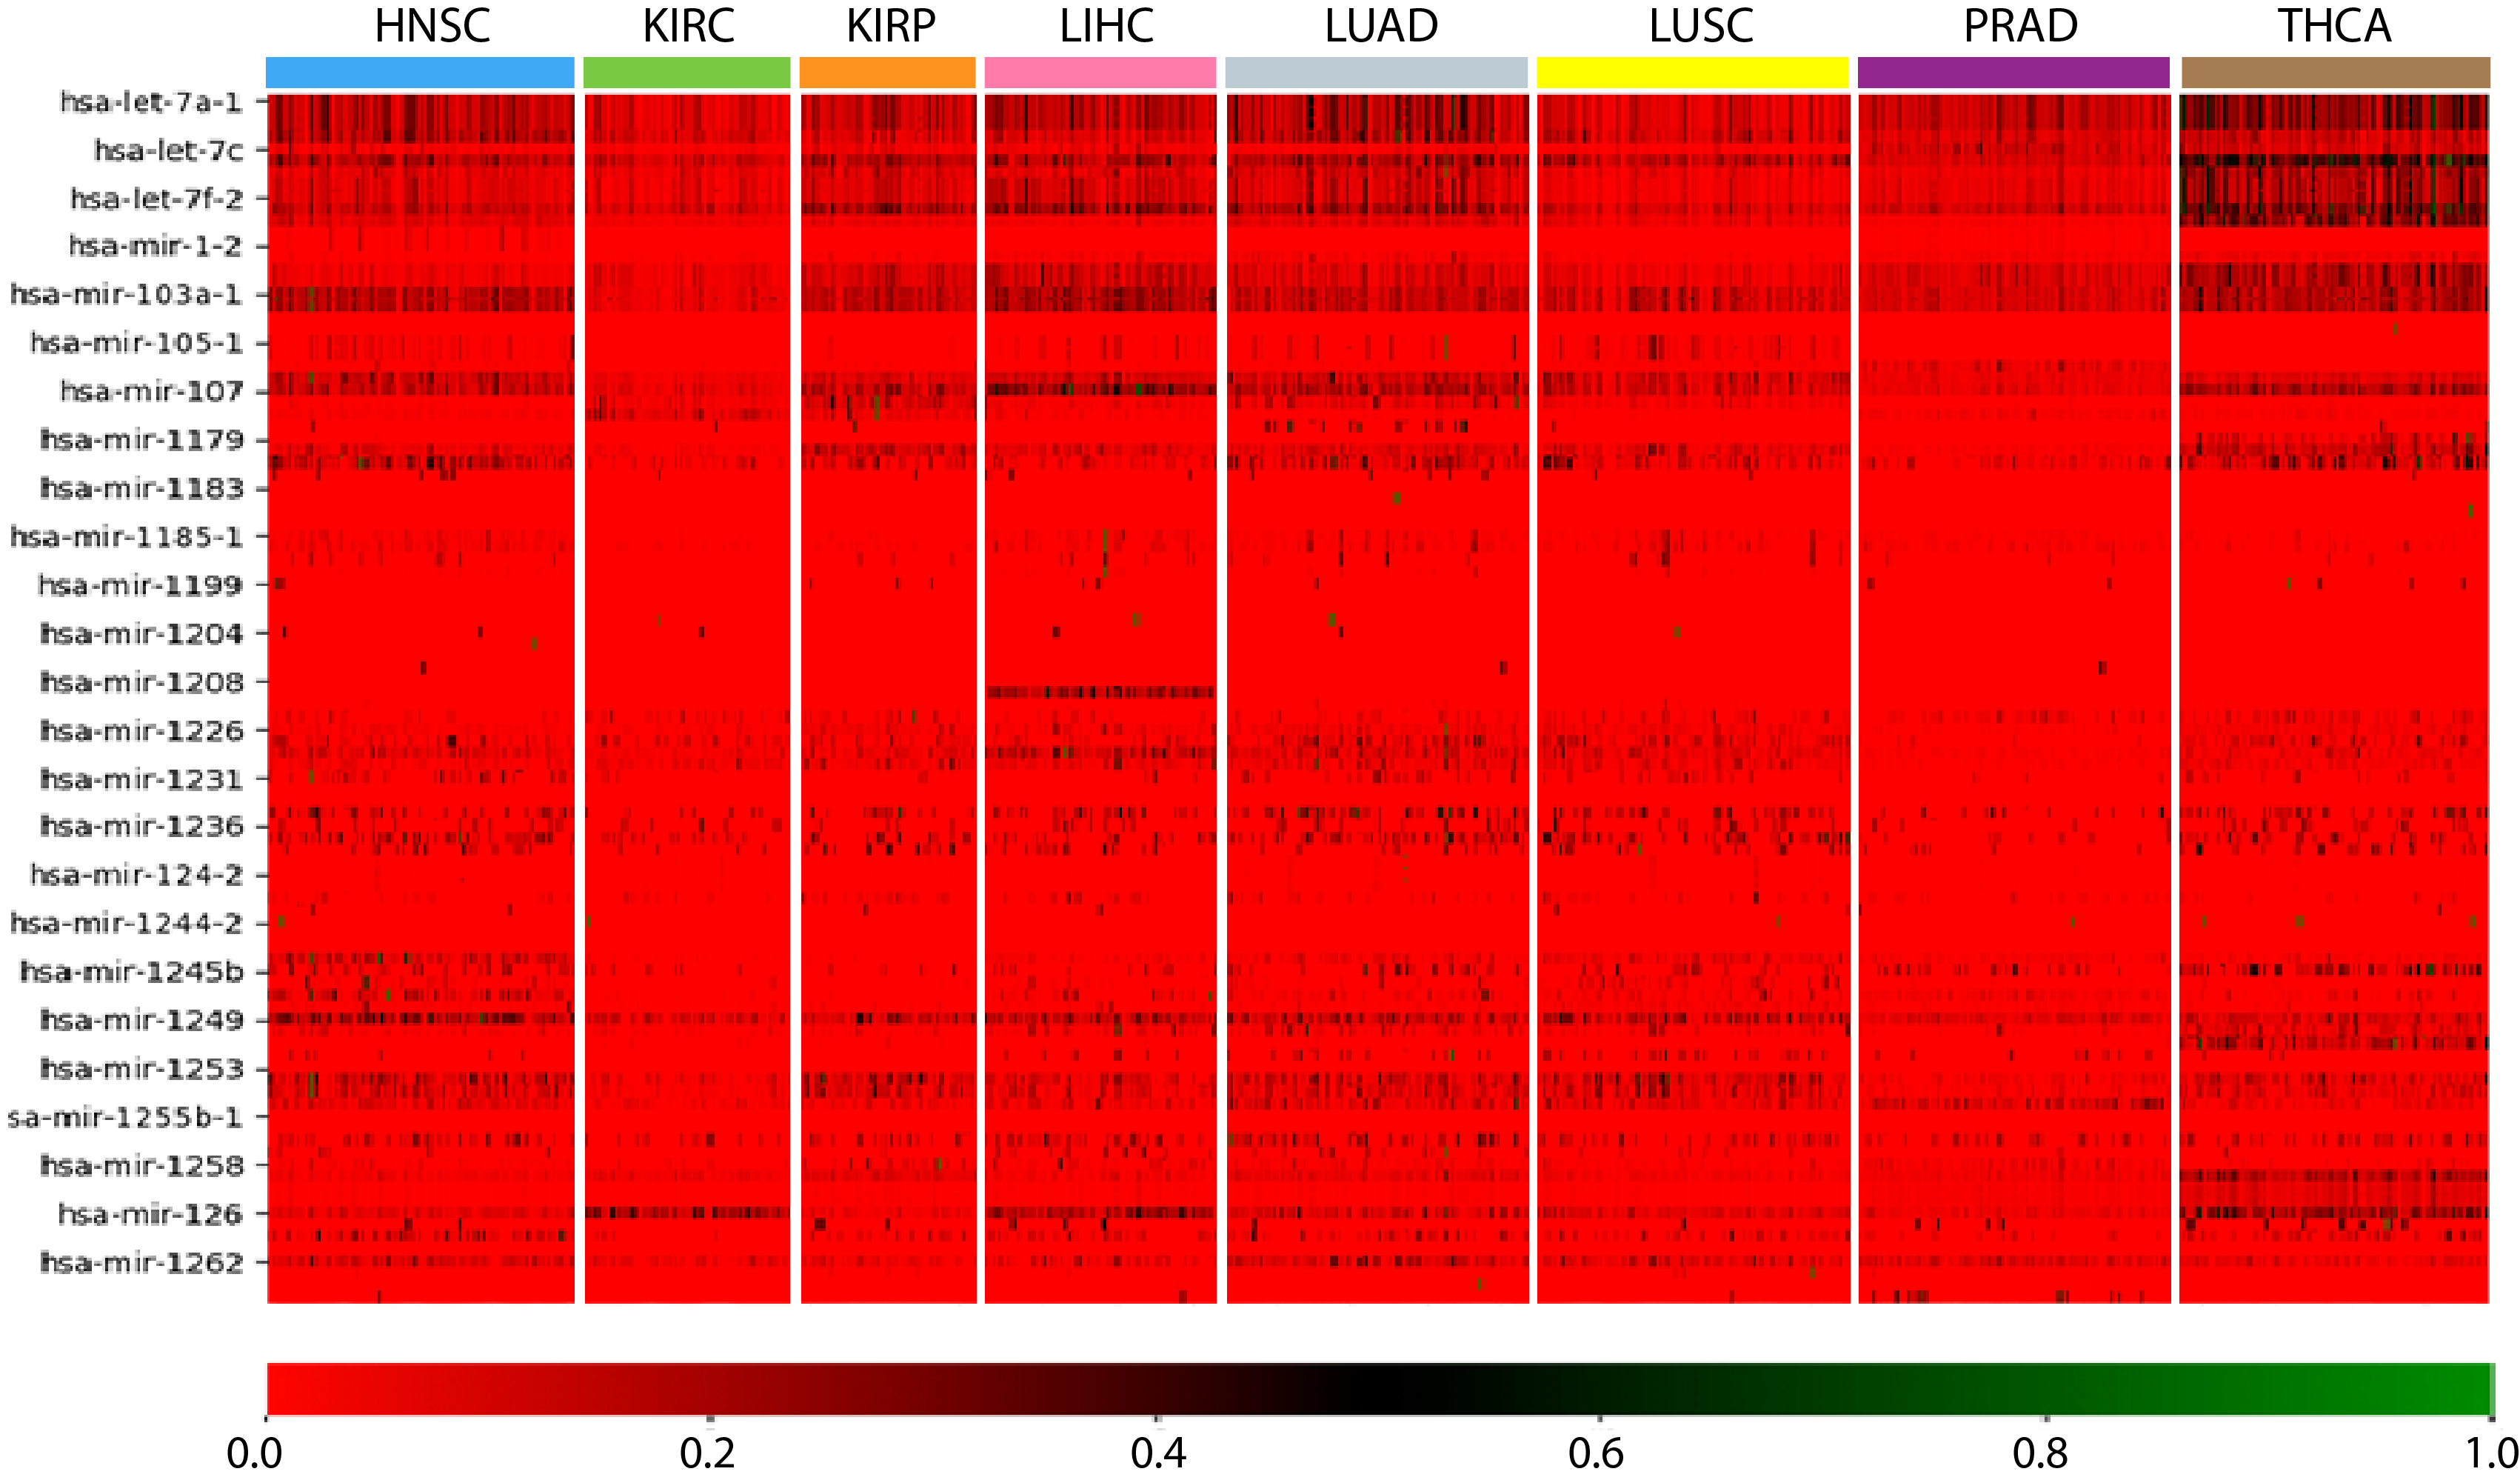
\includegraphics[width=\textwidth]{img/expmirna.png}
    \noindent
    \caption{Normalized miRNA expression profiles.}
    \label{fig:expmirna}
\end{figure}

\subsubsection{Dataset}

The expression profiles of the transcriptome expression data had the input feature dimensionality of all assayed genes and miRNA molecules. The miRNA-seq expression data contained the normalized expression counts of 1881 miRNA molecules, while the RNA-seq expression data contained the normalized expression counts of 60484 genes. As a result, the processed miRNA-seq data produced data matrix $M \in {\rm I\!R}^{1881 \; x \; n}$, and the processed RNA-seq data produced data matrix $R \in {\rm I\!R}^{60484 \; x \; n}$.

\subsection{Simple Nucleotide Variation}

\subsubsection{Preprocessing}

The simple nucleotide variation (SNV) data was obtained in the form of masked somatic mutations, derived from a MuTect2 Variant Aggregation and Masking workflow \cite{cibulskis2013sensitive}. 

\begin{figure}[h!]
    \centering
    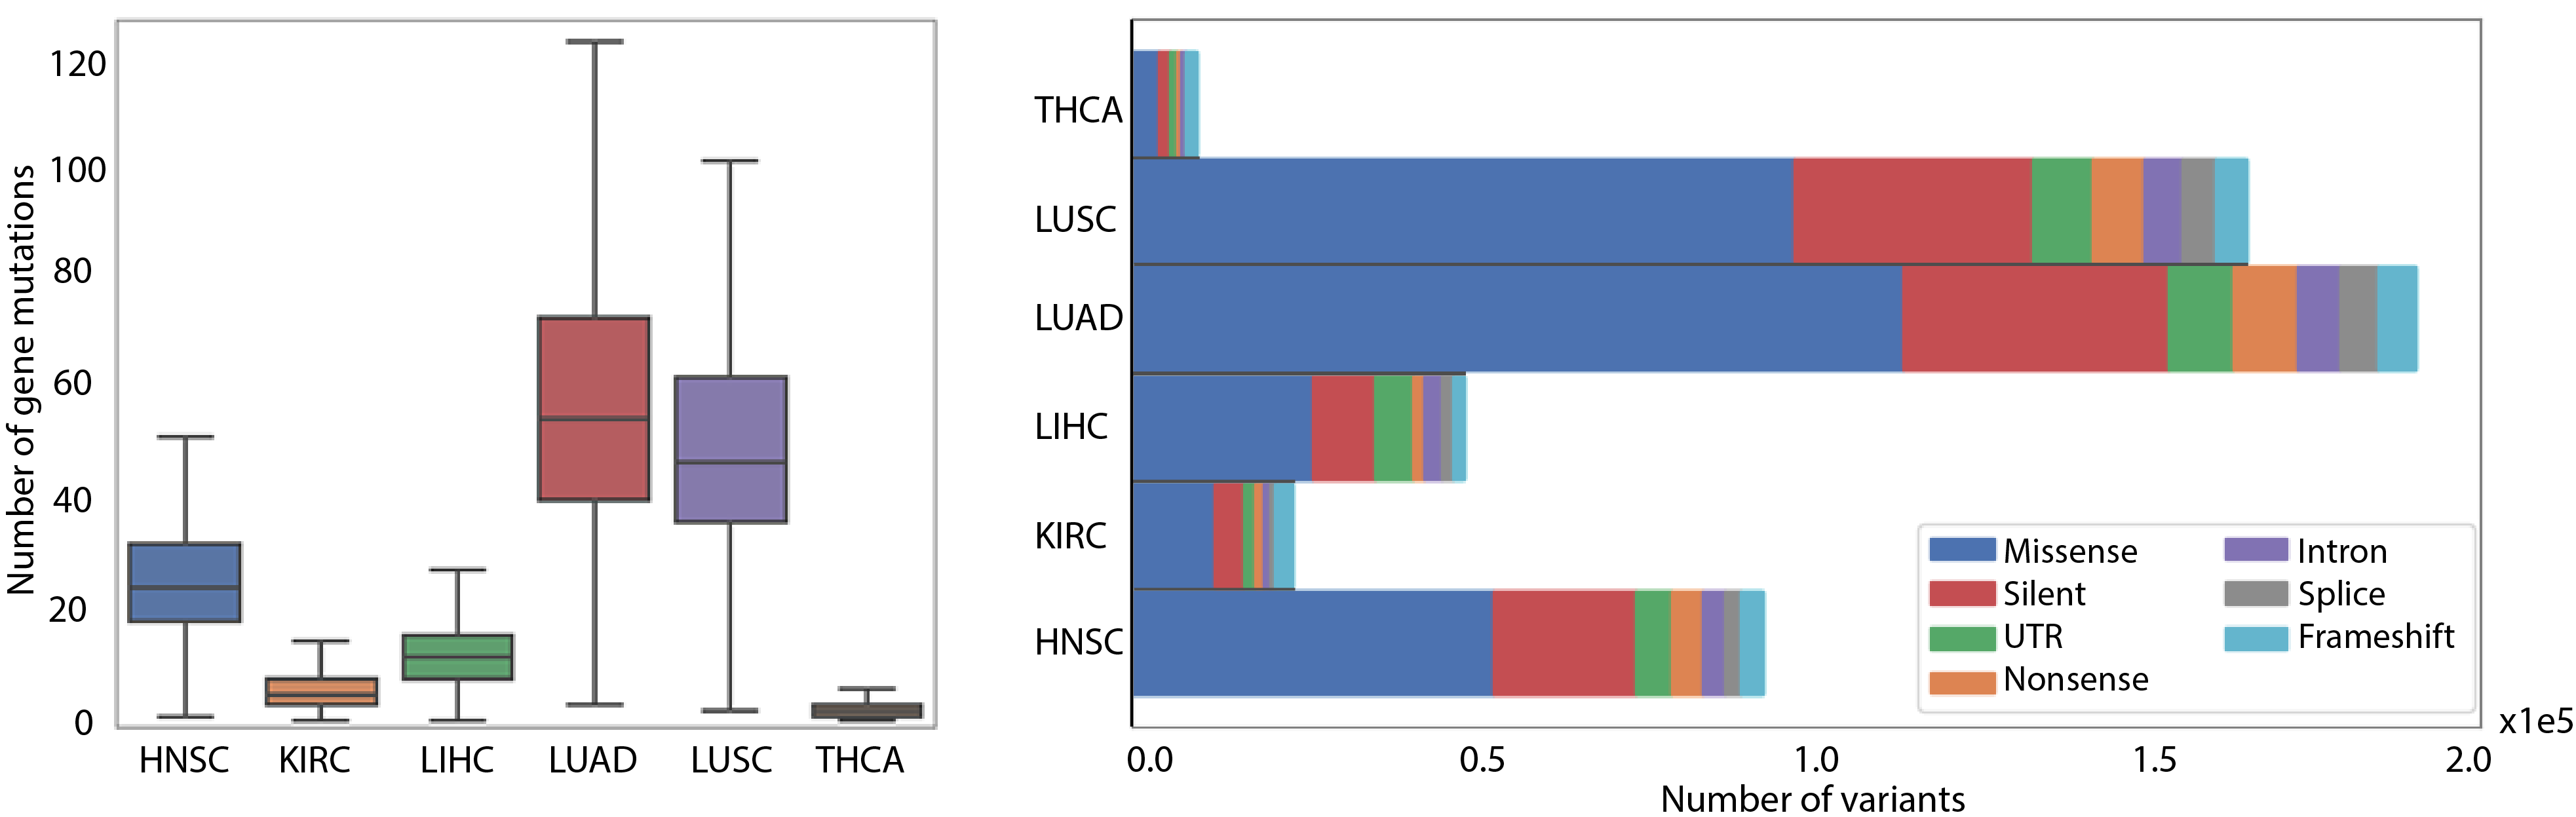
\includegraphics[width=\textwidth]{img/snvstats.png}
    \noindent
    \begin{minipage}[t]{.39\textwidth}
    \raggedright
        a) Accumulated gene mutations
    \end{minipage}% 
    \hspace{1cm}
    \begin{minipage}[t]{.5\textwidth}
        b) Variant classification distribution
    \end{minipage}
    \centering
    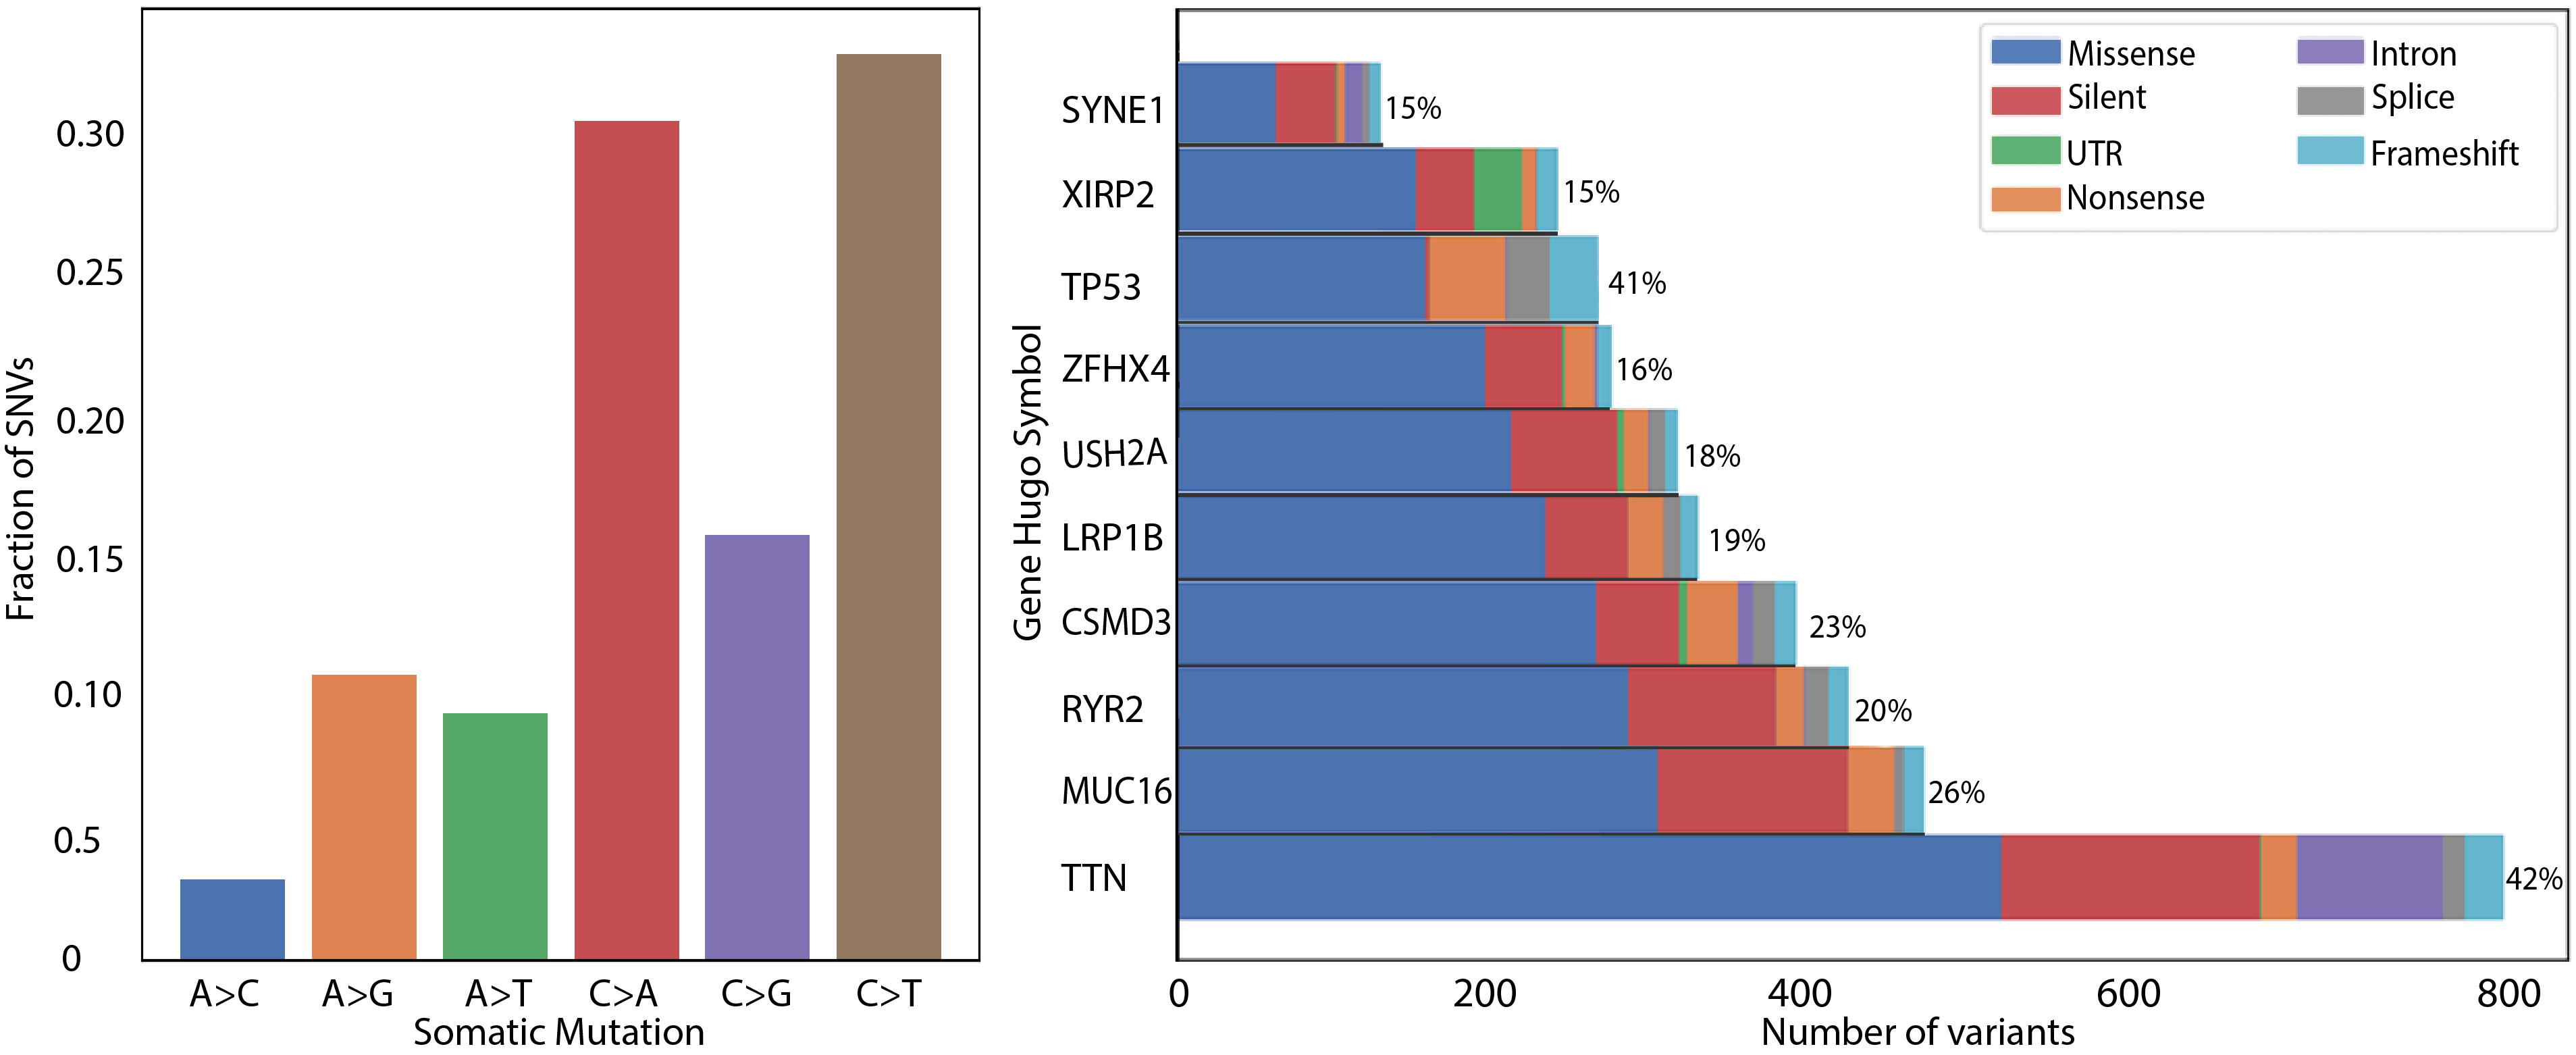
\includegraphics[width=\textwidth]{img/snvstats2.png}
    \noindent
    \begin{minipage}[t]{.39\textwidth}
    \raggedright
        c) Fraction of somatic muations
    \end{minipage}% 
    \hspace{1cm}
    \begin{minipage}[t]{.5\textwidth}
        d) Variant distribution of top 10 mutated genes
    \end{minipage}
    \caption{a) Box plot of accumulated gene mutations for each cancer type. b) Stacked bar plot showing the distribution of variant classification for each cancer type. c) Bar plot showing the fraction of all somatic mutations. d) Stacked bar plot detailing the distribution of the top 10 mutated genes.}
    \label{fig:snvstats}
\end{figure}
%Number of gene mutations per cancer class.



%number of mutations per cancer class vs fraction mutated

In this study, the analysis of the raw SNV data was based on the variant occurrence frequency of thke genetic data. Variation occurence was mapped to every listed gene for all available cell samples. This was performed by mapping mutated genes to cell sample IDs in the raw SNV data, and accumulating the number of mutations for each respective cell sample.

\subsubsection{Dataset}

After preprocessing the SNV data, the variant occurrence frequency was obtained for 20516 human genes for each cell mass sample. The variant occurrence frequency was recorded in matrix $S \in \{\mathbb{Z}_{\geq 0}\}^{20516 \; x \; m}$, where the 20516 rows coorespond to genes, and the m columns correspond to the m cell samples per gene. Accordingly, a field within matrix $S$ indicates the number of mutations observed for a cell on a given gene. 

\section{Dimensionality Reduction}

In the following, we describe the various forms of dimensionality reduction used to deal with the high dimensionality of the genomic data and the selection of relevant features. 

\subsection{Stacked Denoising Autoencoder}

A SDAE was used to acquire compressed feature vectors from all genomic data sources. A two layer SDAE with dimensions 1000, and 500 was trained using a designated training set. Optimal model parameters were selected based on model performance during 10-fold cross validation. Post training, a layer with reduced dimensionality and a low cross validation error was selected. The defined objective here was to acquire a reduced mapping that encodes the original data with minimal loss of meaningful patterns.

\subsection{Deeply Connected Genes}
The weights of the trained SDAE were used to extract the raw features most strongly connected to the reduced subspace for CNV, RNA-seq and miRNA-seq data sources. These features were extracted from the SDAE by computing the product of the weight matrix for each layer \cite{danaee2017deep}. 
The product of the weights for each layer in the trained and optimally parametized SDAEs were observed to be highly normally distributed as shown in Figure \ref{fig:zscoreHist}. 

\begin{figure}[h!]
     \centering
     \begin{subfigure}[b]{0.3\textwidth}
         \centering
         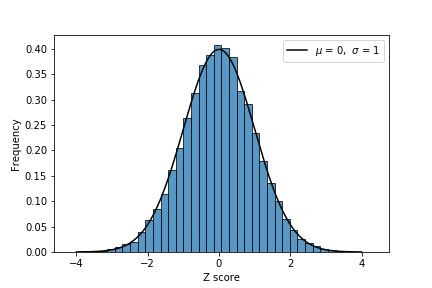
\includegraphics[width=\textwidth]{img/zscoreCNV.png}
         \caption{}
     \end{subfigure}
     \hfill
     \begin{subfigure}[b]{0.3\textwidth}
         \centering
         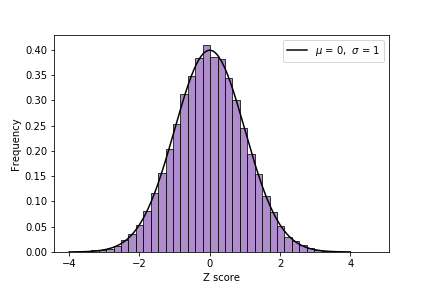
\includegraphics[width=\textwidth]{img/zscoreRNA.png}
         \caption{}
     \end{subfigure}
     \hfill
     \begin{subfigure}[b]{0.3\textwidth}
         \centering
         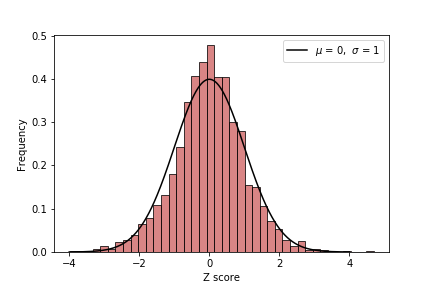
\includegraphics[width=\textwidth]{img/zscoreMIRNA.png}
         \caption{}
     \end{subfigure}
        \caption{Histogram of z-scores from dot product of SDAE weight matrices for a) CNV b) RNA-seq and c) miRNA-seq.}
        \label{fig:zscoreHist}
\end{figure}

The most statistically significant features were identified by fitting the weight matrices to a normal distribution, and computing a p value to select features that match the preselected experimental dimensions.

\subsection{Differential Expression}

For the transcriptome expression data, deferentially expressed genes were identified, and utilized as features. The $log_{2}$(fold change) was computed between the median tumour cell mass expression and healthy cell mass expression. The most statistically significant features were identified by fitting the differential expression to a Guassian distribution and computinbg a two-tailed p-value. Features that match the preselected experimental dimensions were acquired by selected the top most significant deferentially expressed genes using the two-tailed p-values. 

\begin{figure}[h!]
     \centering
     \begin{subfigure}[b]{0.49\textwidth}
         \centering
         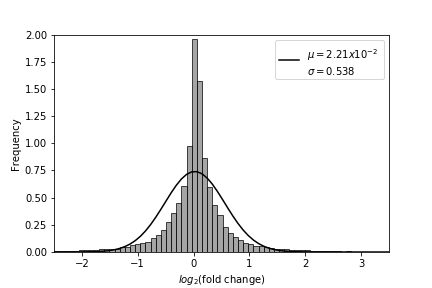
\includegraphics[width=\textwidth]{img/rnaDE.png}
         \caption{}
     \end{subfigure}
     \hfill
     \begin{subfigure}[b]{0.49\textwidth}
         \centering
         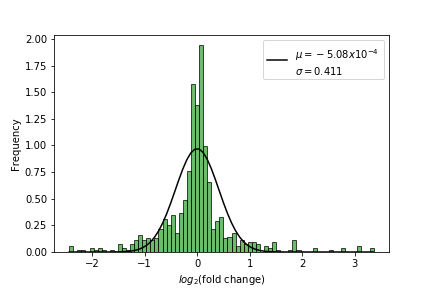
\includegraphics[width=\textwidth]{img/mirnaDE.png}
         \caption{}
     \end{subfigure}
        \caption{Differential expression $log_2$(fold change) and Gaussian fit for a) RNA-seq and b) miRNA-seq.}
        \label{fig:deHist}
\end{figure}
